\documentclass[9pt,]{article}
\usepackage{lmodern}
\usepackage{amssymb,amsmath}
\usepackage{ifxetex,ifluatex}
\usepackage{fixltx2e} % provides \textsubscript
\ifnum 0\ifxetex 1\fi\ifluatex 1\fi=0 % if pdftex
  \usepackage[T1]{fontenc}
  \usepackage[utf8]{inputenc}
\else % if luatex or xelatex
  \ifxetex
    \usepackage{mathspec}
  \else
    \usepackage{fontspec}
  \fi
  \defaultfontfeatures{Ligatures=TeX,Scale=MatchLowercase}
\fi
% use upquote if available, for straight quotes in verbatim environments
\IfFileExists{upquote.sty}{\usepackage{upquote}}{}
% use microtype if available
\IfFileExists{microtype.sty}{%
\usepackage{microtype}
\UseMicrotypeSet[protrusion]{basicmath} % disable protrusion for tt fonts
}{}
\usepackage[margin=1in]{geometry}
\usepackage{hyperref}
\PassOptionsToPackage{usenames,dvipsnames}{color} % color is loaded by hyperref
\hypersetup{unicode=true,
            pdftitle={Cascading effects of critical transitions in social-ecological systems},
            pdfauthor={Juan C. Rocha, Garry Peterson, Örjan Bodin, Simon Levin},
            pdfkeywords={regime shifts, cascading effects, tele-connections, networks},
            colorlinks=true,
            linkcolor=blue,
            citecolor=blue,
            urlcolor=blue,
            breaklinks=true}
\urlstyle{same}  % don't use monospace font for urls
\usepackage{graphicx,grffile}
\makeatletter
\def\maxwidth{\ifdim\Gin@nat@width>\linewidth\linewidth\else\Gin@nat@width\fi}
\def\maxheight{\ifdim\Gin@nat@height>\textheight\textheight\else\Gin@nat@height\fi}
\makeatother
% Scale images if necessary, so that they will not overflow the page
% margins by default, and it is still possible to overwrite the defaults
% using explicit options in \includegraphics[width, height, ...]{}
\setkeys{Gin}{width=\maxwidth,height=\maxheight,keepaspectratio}
\IfFileExists{parskip.sty}{%
\usepackage{parskip}
}{% else
\setlength{\parindent}{0pt}
\setlength{\parskip}{6pt plus 2pt minus 1pt}
}
\setlength{\emergencystretch}{3em}  % prevent overfull lines
\providecommand{\tightlist}{%
  \setlength{\itemsep}{0pt}\setlength{\parskip}{0pt}}
\setcounter{secnumdepth}{0}
% Redefines (sub)paragraphs to behave more like sections
\ifx\paragraph\undefined\else
\let\oldparagraph\paragraph
\renewcommand{\paragraph}[1]{\oldparagraph{#1}\mbox{}}
\fi
\ifx\subparagraph\undefined\else
\let\oldsubparagraph\subparagraph
\renewcommand{\subparagraph}[1]{\oldsubparagraph{#1}\mbox{}}
\fi

%%% Use protect on footnotes to avoid problems with footnotes in titles
\let\rmarkdownfootnote\footnote%
\def\footnote{\protect\rmarkdownfootnote}

%%% Change title format to be more compact
\usepackage{titling}

% Create subtitle command for use in maketitle
\newcommand{\subtitle}[1]{
  \posttitle{
    \begin{center}\large#1\end{center}
    }
}

\setlength{\droptitle}{-2em}
  \title{Cascading effects of critical transitions in social-ecological systems}
  \pretitle{\vspace{\droptitle}\centering\huge}
  \posttitle{\par}
  \author{Juan C. Rocha, Garry Peterson, Örjan Bodin, Simon Levin}
  \preauthor{\centering\large\emph}
  \postauthor{\par}
  \predate{\centering\large\emph}
  \postdate{\par}
  \date{August 31, 2017}

\usepackage{dcolumn}
\usepackage{lineno}
\linenumbers

\begin{document}
\maketitle
\begin{abstract}
Critical transitions in nature and society are likely to occur more
often and severe as humans increase they pressure on the world
ecosystems. Yet it is largely unknown how these transitions will
interact, whether the occurrence of one will increase the likelihood of
another, or whether they might simply correlate on distant places. Here
we present a framework for exploring three types of potential cascading
effects of critical transitions\(:\) drivers sharing, domino effects and
hidden feedbacks. Drivers and feedback mechanisms are reduced to a
directed signed graph that allow us to explore drivers co-occurrence.
Sharing drivers is likely to increase correlation in time or space among
critical transitions but not necessarily interdependence. Domino effects
occur when the feedback processes of one regime shifts affect the
drivers of another, creating a one way dependency. Hidden feedbacks were
identified by mapping circular pathways on coupled networks that have
not been previously reported, helping us detect potential two way
dependencies. The method serves as a platform for hypothesis exploration
of plausible new feedbacks between critical transitions in
social-ecological systems; it helps to scope structural interdependence
and hence an avenue for future modelling and empirical testing of regime
shifts coupling.
\end{abstract}

\subsection{Introduction}\label{introduction}

Critical transitions or regime shifts has been documented on a wide
variety of systems from climate, finance, language, neurological
diseases, ecosystems and ancient societies\textsuperscript{1,2}. A large
set of regime shifts in social-ecological systems has been
identified\textsuperscript{3}; and as human pressures increase on the
planet, these transitions might become more acute and frequent than
previously thought\textsuperscript{4}. Research on regime shifts is
often confined to well defined domains of expertise (e.g.~limnology,
urbanism, climate science), adopting either an empirical,
modelling\textsuperscript{5} or early warnings indicator
approach\textsuperscript{6,7}. These approaches require a deep knowledge
of the causal structure of the system or a high quality spatio-temporal
data respectively. These requirements have confined the body of research
to the analysis of individual types of regime shifts rather than the
potential interactions across systems. Yet, one of the key challenges of
sustainability science is analyzing the diverse set of interactions
across human-environmental systems\textsuperscript{8}.

Regime shifts are large, abrupt and persistent changes in the function
and structure of systems\textsuperscript{9,10}. They present a challenge
for ecological management and governance because they are very difficult
to predict\textsuperscript{11,12} and reverse\textsuperscript{9}, while
having substantial impacts on the availability or ecosystem services
that societies rely upon\textsuperscript{13}. A regime is the region of
the parameter space where state variables (e.g.~vegetation density,
coral cover) fluctuate, they are also called equilibrium, alternative
stable states, basins or domains of attraction. Systems prone to regime
shifts have more than one alternative stable states; under similar
parameter values they can suddenly shift from one domain to another when
critical thresholds are crossed\textsuperscript{14,15}. Change in slow
variables (e.g.~temperature in coral reefs) often shrinks the basin of
attraction, making the system more susceptible to shifting when exposed
to shock events (e.g.~hurricanes) or the action of external
drivers\textsuperscript{6}.

How different regime shifts might be interconnected is largely unknown
and a key frontier of research\textsuperscript{8,16}. Some examples of
cascading effects between regime shifts have been reported in the
literature but a systematic review is lacking. For example,
eutrophication is often reported as a preceding ecosystem state to
hypoxia or dead zones in coastal areas\textsuperscript{17}. Similarly,
hypoxic events have been reported to affect the resilience of coral
reefs to warming and other stressors in the tropics\textsuperscript{18}.
Moisture recycling feedback is a key underlying process on the shift
from forest to savanna\textsuperscript{19,20} or the Indian
monsoon\textsuperscript{21}; but also has the potential to couple
ecosystems beyond the forest that depend on moisture recycling as an
important water source. Changes in moisture recycling can affect
mountain forest in the Andes\textsuperscript{23,24}, nutrient cycling in
the ocean by affecting sea surface temperature and therefore regime
shifts in marine food webs\textsuperscript{25}, or exacerbation of dry
land related regime shifts\textsuperscript{26}. More recently it has
been reported that increasing frequency of boreal forest fire could be
actually strong enough to increase warming in the
Arctic\textsuperscript{27,28}. Permafrost thawing across the Arctic
peatlands can be a dangerous amplifier of global warming too by
releasing methane\textsuperscript{29}. Mangrove forest are expected to
store less carbon as their areas shrink and their ability to build peat
soils is overwhelmed by sea level rise; however it is unclear whether
the effect will be comparable as to impact global carbon budgets and
further warming\textsuperscript{30}. While this growing body of
literature already presents some potential cascading effects, a rigorous
method for systematically assessing what regime shifts could be
interconnected and how is needed.

The aim of this paper is developing a framework for exploring potential
interactions amongst regime shifts in social-ecological systems. We
propose three types of interconnections: \emph{i)} two regime shifts can
sync if they are affected by the same driving
forces\textsuperscript{31}; \emph{ii)} a domino effect is triggered when
the occurrence of one regime shift affects the drivers of other regime
shift\textsuperscript{6,16,32}; or \emph{iii)} when two regime shifts
dynamics generate new (not previously identified) feedback
dynamics\textsuperscript{8} by reinforcing or damping each other
drivers\textsuperscript{32}. Here we present a graphical framework based
on networks to explore such hypothetical interconnections.

\subsection{Method summary}\label{method-summary}

The question we are trying to answer: whether regime shifts might be
interconnected and how - calls for a method for studying relational
data, namely networks. Before outlining the technical details and data
used, first we present the hypothesis we test. Then we describe the
datasets used and how networks help us identify the three types of
interconnections proposed. Last, the statistical analysis tailored to
our networks is presented.

What the examples from the literature mentioned above have in common is
that a larger scale feedback often affects a more localized dynamic in
another ecosystem. However, the opposite is also possible, when the
accumulation of small-scale process scale up and impact larger scale
dynamics. Peters \emph{et al.}\textsuperscript{33} explored under this
line of thinking the dynamics of the dust bowl, desertification, or
amplification of fire dynamics\textsuperscript{26,33}. Therefore our
first hypothesis is that cross-scale dynamics underlie potential
cascading effects: we expect that domino effects will be mostly
dominated by connections between regime shifts that occur in relatively
larger scales and slower dynamics in time towards regime shifts in
smaller scales and faster in time. Conversely, we expect that hidden
feedbacks will occur when scales match (both in space and time), as well
as under similar ecosystem types. We expect that regime shifts occurring
in similar ecosystem types or land uses will be subject to relatively
similar sets of drivers, increasing the likelihood of drivers sharing.
While regime shifts might have similar impacts on ecosystem services and
human well being, we do not expect such similarities to be significant
aspects increasing the likelihood of sharing drivers, domino effects or
hidden feedbacks.

To test these hypotheses we used the \href{www.regimeshifts.org}{regime
shifts database}, to our knowledge the largest online repository of
regime shifts in social-ecological systems (Fig. 1). It offers syntheses
of over \(30\) generic types of regime shifts, \(> 300\) case studies
based on literature review of \(> 1000\) scientific
papers\textsuperscript{3}. The database decomposes regime shifts in
terms of describing their regimes, drivers, feedback mechanisms, impacts
on ecosystem services, and management options. It provides a set of
\(92\) categorical variables about impacts, scales, and evidence
type\textsuperscript{3}. When possible, entries to the regime shifts
database have been peer reviewed by an expert on the topic to ensure
quality and accuracy of its contents\textsuperscript{3}. The regime
shifts database also offers causal loop diagrams as a summary of the
driving processes and underlying feedbacks of regime shifts. Each causal
loop diagram was turned into a network by creating the adjacency matrix
\(A\), where \(A_{i,j}\) is \(1\) if there is a connection or zero
otherwise. Link sign \(w_{i,j}\) represent link polarity taking \(-1\)
if the relationship is expected to be inverse proportional, or \(1\)
when proportional (See SM). Based on the signed graphs we created three
response variables corresponding to each of the cascading effects.

Our hypotheses were tested using as response variable for \emph{drivers
sharing} the number of drivers shared, for \emph{domino effects} the
number of directed pathways that connect two regime shifts, and for
\emph{hidden feedbacks} it is the number of k-cycles that emerge on the
joined network that do not exist on the separate causal networks (See
SM). Note that all three response variables are matrixes that can be
represented as weighted networks in our statistical framework where
nodes are regime shifts and the link depends on the cascading effect
described. Our research question can be translated then to what is the
likelihood of a link between regime shifts in this network, and what
features change this likelihood. The explanatory variables (such as
scale) are modeled as edge covariates derived from the regime shifts
categorical variables (\(N=92\), See SM). We focused on how similar two
regime shifts are -regarding the categorical variables they share- and
how that similarity increases or not the likelihood of having a link,
this is, the likelihood of presenting any of the cascading effects
types. All these networks contain all valued links of count data,
therefore the specification for the exponential random graph models
follows Krivitsky\textsuperscript{34} and a Poisson reference
distribution. We also fitted ordinary least squares OLS approximation
that only takes similarity, not network structure, into account. All
software used is under open access license\textsuperscript{35--38} and
run under the R statistical language\textsuperscript{39}.

\begin{figure}

{\centering 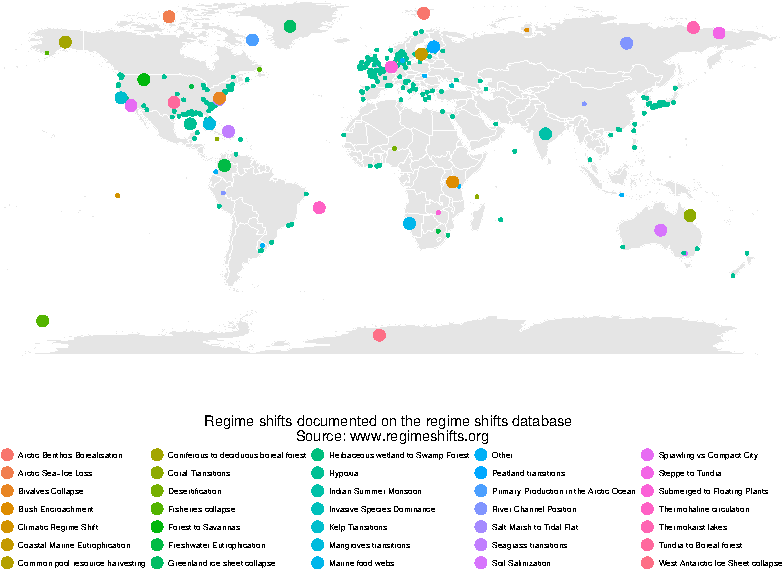
\includegraphics{170830_draftCascadingEffects_files/figure-latex/Fig1-1} 

}

\caption{Regime shifts around the world. Large points show generic types of regime shifts (n = 35) while small points are case studies (n=324).}\label{fig:Fig1}
\end{figure}

\begin{figure}

{\centering 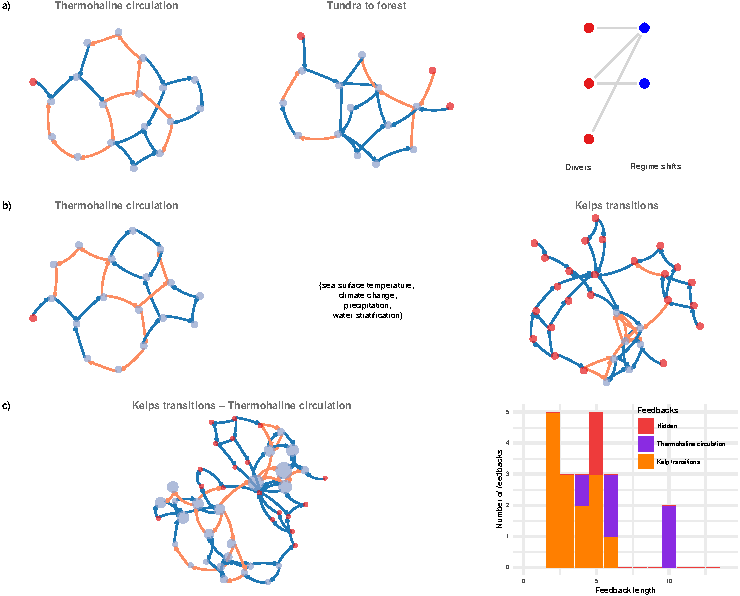
\includegraphics{170830_draftCascadingEffects_files/figure-latex/Fig2-1} 

}

\caption{Minimal examples of the cascading effects framework. a) Sharing drivers: Causal loop diagram examples for the regime shift on the thermohaline circulation and tundra to forest. Positive links are depicted as blue arrows, negative links as orange arrows, drivers are variables outside feedback loops (in red), while variables inside feedbacks are grey. While thermohaline circulation has one driver, tundra to forest has three. The bipartite network (right) depicts drivers (red nodes) shared by these two regime shifts (blue nodes), the only driver shared by both is green house gas emissions. b) Domino effects: Four variables are part of feedback processes in the causal loop diagram of thermohaline circulation that are in turn drivers of kelps transitions. Domino effects create directional dependencies between regime shifts. c) Hidden feedbacks: Both causal loop diagrams in b) are merged into a network where both links and node sizes are scaled according to the number of feedback loops where they are involved. The histogram on the right shows the number of feedbacks per feedback length. Hidden feedbacks are feedbacks that emerge when joining the networks that did not exist on the individual regime shift networks, in this example two hidden feedbacks exist of length 5.}\label{fig:Fig2}
\end{figure}

\subsection{Results}\label{results}

\begin{figure}

{\centering 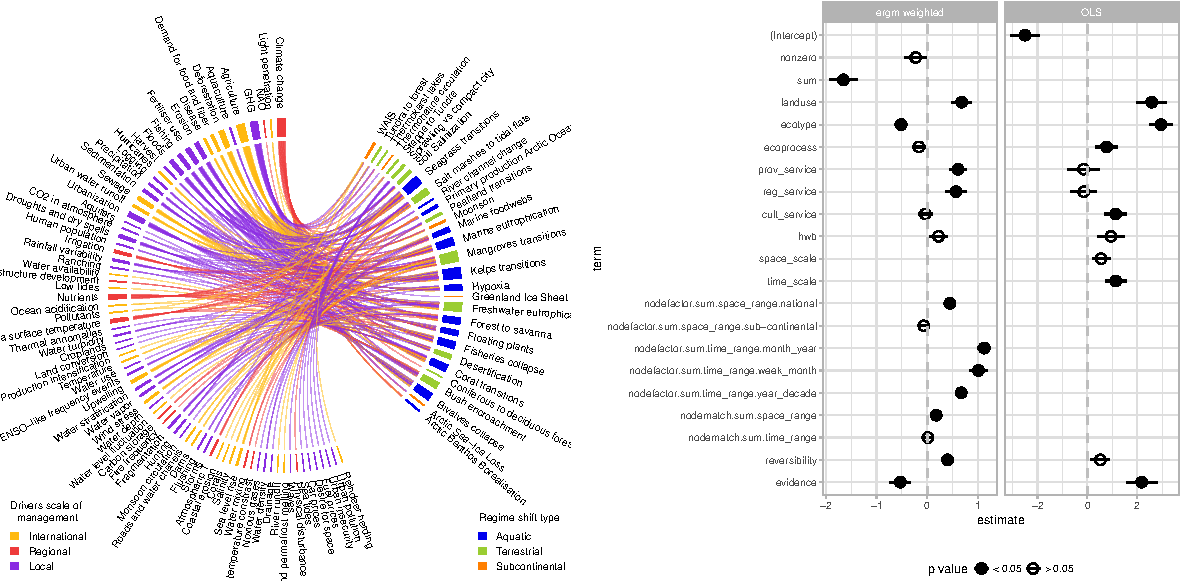
\includegraphics{170830_draftCascadingEffects_files/figure-latex/Fig3-1} 

}

\caption{Bipartite network of sharing drivers shows fork type of cascading effects. Updated version from Rocha et al (2015) with 30 regime shifts. WAIS stands for West Antarctica Ice Sheet collapse, NAO is North Atlantic Oscillation, and GHG is green house gases.}\label{fig:Fig3}
\end{figure}

Drivers sharing were investigated by creating a bipartite graph - a
network with two type of nodes (Fig. 2a) - linking drivers nodes to
regime shifts nodes if there is a reference in the scientific literature
suggesting causality\textsuperscript{31}. This type of connection is
expected to increase the likelihood of synchronization in space and time
of different regime shift phenomena\textsuperscript{16} (correlations),
both in terms of cases (e.g.~two different coral reefs) or regime shift
types (e.g.~thermokrast lakes and peatland transitions both driven by
climate change). A preliminary exploration of \emph{drivers sharing} was
introduced by Rocha \emph{et al.}\textsuperscript{31} when asking the
question of what are the main drivers of regime shifts globally. While
their focus was on drivers importance, here we updated their analysis to
30 regime shifts and focus on what aspects increase the likelihood of
two regime shifts sharing the same drivers. Figure 3 presents the
bipartite network composed by 79 drivers and 30 regime shifts. Regime
shifts in this network are more likely to share drivers when they occur
on similar ecosystem types and impact similar regulating services (p
\textless{}\textless{} 0.001, SM Tables 1,2). The odds of two regime
shifts sharing drivers is 0.8, while the odds of them sharing drivers
given that they occur on similar ecosystem type is 0.48. The likelihood
of sharing drivers is also affected by occurring on similar land use,
impacting similar cultural services and aspects of human wellbeing,
occurring at similar spatial scales (but not temporal ones), as well as
having similar types of evidence and reversibility (p \textless{} 0.05,
SM Table 2). Interestingly, while the likelihood of having a non-zero
link is significant, the number of drivers shared is not. The negative
coefficient on the \texttt{non-zero} term indicates zero inflation, this
is that most of the interaction occur through the link weights as
opposed to the number of links, confirming previous
results\textsuperscript{31} for clustering coefficient and co-occurrence
index on the bipartite network. The naïve OLS approach render slightly
similar results, while reversibility, provisional and regulating
services are not significant, similarity on temporal scales is
correlated to number of drivers shared. Yet, the amount of variance
explained by the OLS model is relatively low (adjusted \(R^2\)
\textasciitilde{} 0.3), while the AIC and BIC for the model that
consider network structure and regime shifts attributes is much better
than the null model with network structure alone (SM Table 2).

Domino effects were investigated by searching variables that belong to
feedback mechanisms in one regime shift and at the same time can be
drivers of another (Fig 4, see a worked example in Fig 2b). While most
of pair-wise combinations of regime shifts do not have pathways that can
result on domino effects, the maximum number of pathways found was
\(4\). In line with our expectations, regime shifts that contain
variables that will in turn be drivers of other regime shifts typically
have large spatial scales and slow temporal scales: thermohaline
circulation collapse, river channel change, monsoon weakening, and
Greenland ice sheet collapse. On the other hand, regime shifts that
receive the influence are often marine and their time and space dynamics
contained more locally: kelps transitions, marine eutrophication,
mangroves transitions, coral transitions and fisheries collapse. The
statistical models support this observation: regime shifts whose time
scale are on the rage of weeks to months are more likely to receive
influence from regime shifts whose dynamics occur on the scale of years
to decades (p \textless{} 0.1), but we did not find evidence for spatial
scale (Table SM2). Both, having a link and having a high number of
pathways are significant (p \textless{} 0.01). Surprisingly, the odds of
having higher numbers of domino effects are increased when regime shifts
impact similar regulating services and similar aspects of human well
being (p \textless{} 0.001). The OLS approach pick up weak signals for
ecosystem type and reversibility (p \textgreater{} 0.01) but without the
network structure the power of the OLS model is low (adjusted
\(R^2= 0.018\)). The exponential random graph model that consider both
network structure and regime shifts attributes is much better than the
null model with network structure alone (SM Table 3).

\begin{figure}

{\centering 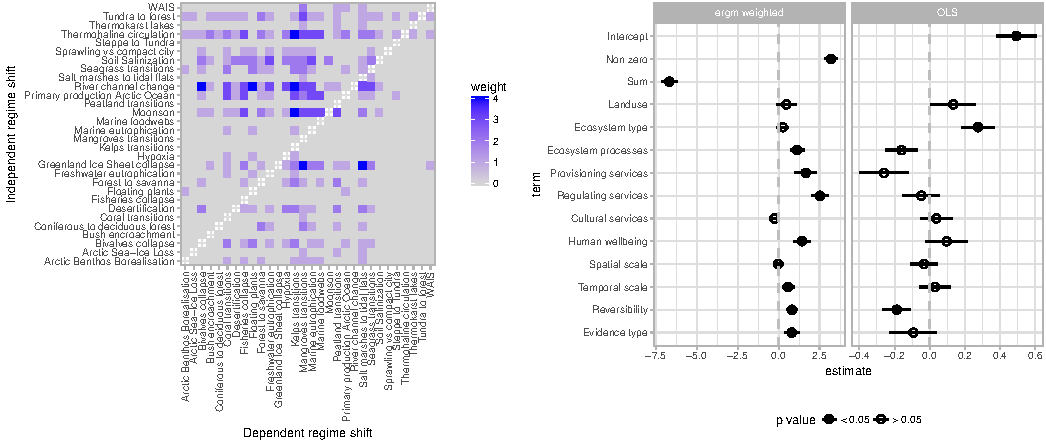
\includegraphics{170830_draftCascadingEffects_files/figure-latex/Fig4-1} 

}

\caption{Domino effects.}\label{fig:Fig4}
\end{figure}

Hidden feedbacks are feedback loops that might connect two different
regime shifts; and if strong enough, it could amplify or dampen the
coupled dynamics (Fig 2c). A hidden feedback occurs when the dynamics of
one regime shift affects a variable that belongs in turn to another
regime shit and vice versa. In order to identify hidden feedbacks we
merged causal networks (See SM) and found that most feedbacks occur at
higher feedback length (Fig 5). Not all regime shifts are connected by
hidden feedbacks, but when new feedbacks do occur they tend to be on the
right side of the distribution at longer cycle lengths. Even for small
networks, the number of cycles tend to increase exponentially with
respect to the increase of links. Although computationally intensive,
the search for k-cycles is feasible in our networks given the small size
and relative sparse structures. In fact, the maximum cycle length \(k\)
is bounded by the size of the network. Out of the 435 coupled networks
analysed, the maximum feedback length was 56. The statistical analysis
shows that there is a zero inflation on the resulting matrix (fewer
links that one would expect by random), but when they do occur, the odds
of having multiple feedbacks coupling two regime shifts is 7.33 times
higher. The odds of two regime shifts been connected through hidden
feedbacks increase if the pair of regime shifts occur in similar land
uses, impact similar ecosystem processes, impact similar regulating and
cultural services, and if they occur on similar scales in space and time
(Fig 5, SM Table 4, p \textless{} 0.001).

\begin{figure}

{\centering 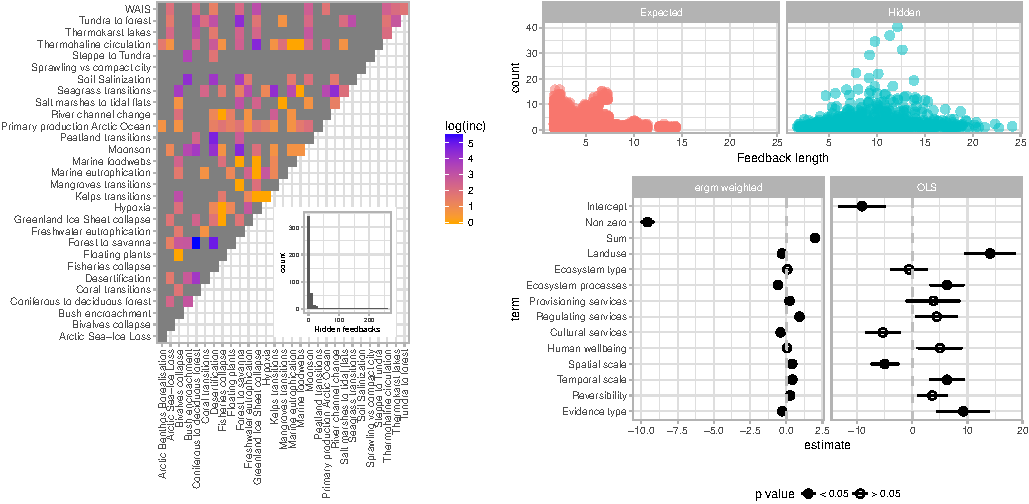
\includegraphics{170830_draftCascadingEffects_files/figure-latex/Fig5-1} 

}

\caption{Hidden feedbacks.}\label{fig:Fig5}
\end{figure}

\begin{figure}

{\centering 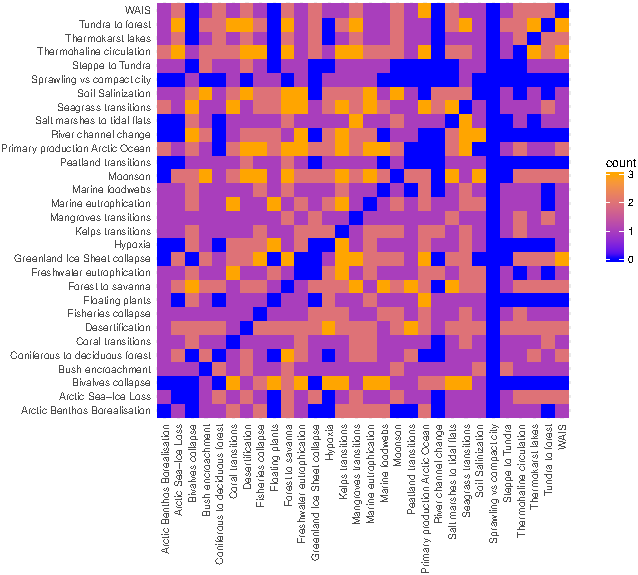
\includegraphics{170830_draftCascadingEffects_files/figure-latex/Fig6-1} 

}

\caption{Cascading effects. Potential identified connections between regime shifts}\label{fig:Fig6}
\end{figure}

\subsection{Discussion}\label{discussion}

This paper aimed to develop a framework for exploring potential
cascading effects among critical transitions in social-ecological
systems. A graphical approach allows us to treat regime shifts as causal
networks composed by feedback mechanisms and drivers reported in the
regime shifts database. Regime shifts interactions can occur when
\emph{sharing drivers}, or when \emph{domino effects} or \emph{hidden
feedbacks} are strong enough to couple their dynamics. While their
dynamic behaviour is outside the scope of this paper, the topological
features that would allow coupling are explored here and serve as a
conceptual devise for hypothesis exploration and further modeling of
this coupled dynamics.

In summary, we have identified structural dependencies that can give
rise to cascading effects among different regime shifts. We hypothesised
that the likelihood of sharing drivers increased when regime shifts
occur on similar ecosystem types and land uses. We confirmed this
observation and also found that sharing drivers increase when regime
shifts occur on the same spatial scales, or when they impact similar
regulating services, cultural services, or impact similar aspects of
human well being. Based on examples of cascading effects already
reported in the literature we hypothesised that domino effects will be
more common between regime shifts whose dynamics occur at larger spatial
scales and slower dynamics in time towards regime shifts more localized
in space and faster in time. We only found support for the cross-scale
dynamic in time but not in space. Additionally, regime shifts that often
received the domino effect tend to occur in aquatic environments
pointing out the importance of water transport as a potential mechanism
linking regime shifts in one-way interacitons. Last, we hypothesised
that hidden feedbacks would appear when scales match both in space and
time, as well as under similar ecosystem types. Our results confirm both
speculations and also suggest that hidden feedbacks are common when
regime shifts occur under the same land use and when they impact similar
ecosystem processes, regulating and cultural services. Figure 6
summarizes the results of our exploration by indicating how many of
these types are plausible. While regime shifts in cities (sprawling
versus dense growth) is not reported to be affected by any cascading
effect with the regime shifts in our dataset, other regime shifts such
as kelps transitions are often subject to the three types of cascading
effects. Of particular importance, the weakening of the Indian Monsoon,
primary production in the Arctic ocean, seagrass transitions, soil
salinization, bivalves collapse and the weakening of the thermohaline
circulation are regime shifts that are expected to be involved in many
of these couplings, at least at the structural level.

Intuitively, the sharing of drivers is proposed as a potential
mechanisms that can correlate regime shifts in space and time, but not
necessarily make them interdependent; unless they also share feedback
mechanisms. Time correlation is debated given that spatial heterogeneity
can break the synchrony induced by the sharing of
drivers\textsuperscript{16}, meaning that contextual settings matter for
such correlations to emerge. Spatial heterogeneity is also attributed as
mechanism that can smooth out critical transitions and soften their
abruptness\textsuperscript{40,41}. Yet, with or without masking
mechanism, identifying common drivers is useful for designing management
strategies that target bundles of drivers instead of well studied
variables independently, increasing the chances that managers will avoid
several regime shifts under the influence of the same sets of
drivers\textsuperscript{31,42}. For example, management options for
drivers such as sedimentation, nutrients leakage, and fishing can reduce
the likelihood of regime shifts in coastal brackish lagoons such as
eutrophication and hypoxia, as well as coral transitions in adjacent
coral reefs.

Domino effects and hidden feedbacks are often disregarded because
research on regime shifts usually focus on one system at the time; data
collection and hypothesis testing for coupled systems has largely
remained unexplored. In fact, the question of how different regime
shifts might be interconnected remains a key frontier of
research\textsuperscript{8,16}. Recent literature report potential
likages between euthrophication and hypoxia\textsuperscript{17}, hypoxia
and coral transitions\textsuperscript{18}, or shifts in coral reefs and
mangroves transitions\textsuperscript{30}. Other examples in the
terrestrial rehalm report potential increase in Arctic warming from
higher fire frequency in boreal forest\textsuperscript{27,28} or
permafrost thawing\textsuperscript{29}, potentially impacting any regime
shift in the Arctic driven by temperature\textsuperscript{43}. Shifts in
forest that can reduce moisture recycling has also been reported to
potentially impact mountain forest\textsuperscript{23,24},
drylands\textsuperscript{26}, and regime shifts in the ocean affected by
nutrients cycling\textsuperscript{25}. While this handful of examples
represent an emergent literature on regime shifts interactions, the
framework here developed allow us to explore more rigorously the type of
potential couplings between regime shifts. For our sample of 30 regime
shifts reported in the regime shifts database, 435 possible pair-wise
combinations exist. Exploring such search space is not a trivial task.
Once the mechanisms responsible for one coupling is identified, it still
remains to be explored the parameter space under which the coupling is
feasible. In other words, while the framework identifies plausible
connections, modeling efforts and observational studies are imperative
to distinguish plausible from probable. While the literature continue to
provide examples of potential couplings, our results contribute to the
ongoing debate by distinguishing whether the coupling is expected to be
correlational because of drivers sharing, a one-way causation (the
\emph{domino effect}), or a two-way interaction (the \emph{hidden
feedbacks}), providing a useful set of hypotheses for future research.

Our analysis is purely topological, it shows what potential domino
effects or feedbacks could exist, but it does not reveals whether the
connection is strong enough to couple the dynamic behaviour of systems
known to be prone to regime shifts. While experimentation is rarely an
option for testing this large scale ecosystem dynamics, observational
studies are of prime importance as well as modeling efforts. Dynamic
models of this type of dynamics require careful assumptions about
parameter values as well as functional form of the system's equations.
Alternatively, generalized modeling is a promising technique that does
not require particular assumptions allowing the researcher to reach more
general conclusions based on the systems
Jacobian\textsuperscript{44--46}. Another potential avenue for future
research is looking at how transport mechanisms couple far apart
ecosystems. One example already mentioned is the moisture recycling
feedback and how it can affect the water budget of areas down the
`\emph{preceipitationshed}'\textsuperscript{47}. Another
teleconneciton\textsuperscript{8} could be with allocation of resources
through international trade, investigating how demand of resources in
certain countries can shape the state space of ecosystems from the
providing countries.

\subsection{Conclusion}\label{conclusion}

Non-linear dynamics are ubiquitous to a large range of social-ecological
systems. However, how a regime shift somewhere in the world could affect
the occurrence of another regime shift remains an open question and a
key frontier of research. Here we have developed a graphical framework
to explore potential cascading effects amongst regime shifts. Based on
topological features of causal networks three type of connections have
been proposed. Potential correlations can arise when regime shifts share
common drivers. While the spatio-temporal correlation can be masked by
heterogeneity or noise, the cluster of drivers shared serves to design
managerial strategies. One-way directional interactions are denoted as
\emph{domino effects} and are common but not exclusive to aquatic regime
shifts. These connections tend to emerge between regime shifts whose
dynamics occur at larger spatial scales and slower temporal scales and
regime shifts in more localized and faster dynamics. Two-way
interconnections are denoted \emph{hidden feedbacks} and occur often
between regime shifts at similar spatio-temporal scales and similar
ecosystem types. The two later types of cascading effects call for a
more holistic approach for modeling and studying regime shifts,
acknowledging their potential interdependences.

\pagebreak

\subsection{Supplementary material}\label{supplementary-material}

This section complements the methods and results of linear regressions
and exponential random graph models. Both modeling techniques used the
number of drivers shared, the number of domino effects and the number of
hidden feedback as the three key response variables. While the linear
regression only takes similarity (calculated with a Jaccard distance on
the attributes coded in the regime shifts database), the exponential
random graph models take into account network structure. Thus, the
latter investigates the odds of the existance and weight of a link.

\subsubsection{Leftovers from the text to edit or
delete:}\label{leftovers-from-the-text-to-edit-or-delete}

The concept of cascading effect has been used in two seemingly different
contexts: i) when referring to the effect of an abrupt change on one
species spreading through food webs\textsuperscript{48,49}; and ii) when
local interactions are magnified by feedbacks that are reinforced across
scales (e.g.~erosion or fire)\textsuperscript{26,33}. What these
interpretations have in common is that both refer to networked systems
(e.g.~foodwebs, landscape mosaics) where a signal (e.g.~fire, species
collapse, disease) spreads broadly or is contained locally depending
upon the system's connectivity. The units of these networks are usually
species or sets of spatial units that represent ecosystems. Here we
broaden the cascading effects concept to networks of regime shifts, when
regime shifts can be represented as causal networks of drivers and
underlying feedback mechanisms or processes (see methods).

\subsubsection{Supplementary methods:}\label{supplementary-methods}

\emph{Causal loop diagrams} (CLDs) represent a collection of causal
mechanisms that scientist have reported in their narratives: both
empirical (what they choose to sample) or theoretical (what they choose
to model). CLDs consist of variables connected by arrows denoting causal
influence\textsuperscript{50}, also known as signed directed graphs.
Each relationship must have a positive \((+)\) or negative \((-)\) sign
that represents the effect of the dependent variable given change on the
independent variable\textsuperscript{50,51}. Although the functional
form that underlies each relationship is not necessarily known, positive
relationships are proportional while negative are inverse proportional
\emph{ceteris paribus}. CLDs assume that the causal relationships
captured by links are monotonic, while non-linearities are captured by
links sets, thus they do not have self-loops. Feedback loops are the
basic structural units of the diagram and emerge by connecting variables
in closed directed paths (cycles). Feedback means that once a signal
enters the loop, some part of the output is feed back to the input,
resulting on amplification or dampening of its own signal. Feedbacks can
be reinforcing if the overall polarity of its links is positive, or
balancing if negative. Reinforcing feedbacks are usually responsible for
behaviours that drives the system out of equilibrium, while balancing
feedbacks are responsible for near equilibrium dynamics such as
oscillations and delays\textsuperscript{50}. Note that causal links do
not describe the behaviour of variables, only the structure of the
system: they describe what would happen if there were
changes\textsuperscript{50}. CLDs were curated in the regime shifts
database in a way that variables names are consistent (e.g.~agriculture
and cropping is kept as `agriculture'), and feedback loops comparable
(e.g.~albedo in the rainfores, Arctic or Antarctic regime shifts is the
same feedback).

\emph{Categorical variables:} We calculated the similarity of each
pair-wise combination of regime shifts in the database regarding
categorical attributes such as \emph{(i)} land use under which the
regime shift occur, \emph{(ii)} ecosystem type, impacts on \emph{(iii)}
ecosystem processes, \emph{(iv)} provisioning services, \emph{(v)}
regulating services, \emph{(vi)} cultural services, \emph{(vii)} and
human wellbeing; as well as \emph{(viii)} the spatial scale at which the
regime shift occur, \emph{(ix)} the temporal scales, \emph{(x)}
reversibility, and \emph{(xi)} evidence type\textsuperscript{3,31}. For
all \(92\) categorical variables encoded, the database reports presence
or absence \((0,1)\) allowing us to calculate the Jaccard index and use
it as a proxy of how similar two regime shifts are. To facilitate the
interpretation of statistical models, the Jaccard distance was rescaled
(\(x =1 - J_{d}\)) so equivalent regime shifts score 1 and complete
dissimilar zero. Given that most of our hypothesis relate to the scale
at which regime shifts occur, we also modeled scale as a categorical
variable to account for matches in the network, no only similarity.

\emph{Networks:} Causal loop diagrams were reinterpreted as networks
where node attributes were coded if a node belongs to a feedback loop -a
k-cycle in the network- or not. The later is then by definition a
driver, an independent variable whose dynamics are not affected by the
dynamics of the state variables of the system at hand. Note that
networks in ecology usually describe inter species interactions such as
predation or mutualism. Our approach is different from what has been
done in ecology. Here a network describe a set of processes, both biotic
and abiotic, that can govern ecosystem regime shifts dynamics. Our
approach is inspired by other network applications to processes such as
cells metabolic networks or the network of human diseases, where a
process is not captured by a link type (e.g.~predation) but by a
collection of link interactions (e.g.~the Krebs cycle). Thus, individual
species are not taken into consideration, but rather their functional
role at the aggregated ecosystem scale (e.g.~herbivory).

\emph{Shared drivers:} To study shared drivers we created a bipartite
network of drivers and regime shifts following the method outlined by
Rocha et al\textsuperscript{31}. The statistical models were performed
for the case of drivers sharing on the one-mode network projection of
regime shifts sharing drivers (this is the matrix \(A^TA\)), and
categorical variables from the regime shifts database were used as node
attributes or node covariates to test our hypothesis.

\emph{Domino effects:} occur when the occurrence of a regime shift can
increase or decrease the likelihood of other regime shift occurring,
creating a one-way dependence. Different from the driving sharing
network, here we explore potential domino effects by using the full
causal loop diagrams as networks. The algorithm for identifying domino
effects takes the adjacency matrix of two given regime shifts \(A_1\)
and \(A_2\) and identifies all nodes \(n \in A_1 \cap A_2\) such that
\(n\) belong to a feedback in \(A_1\) but is a driver in \(A_2\). Thus,
set differences between causal pathways suggest missing drivers, and set
intersection between causal pathways and feedback loop nodes indicate
potential domino effects (Fig. 2b). By iterating this simple algorithm
we derived how many different pathways exist between every pair-wise
combination of regime shifts \((N=435)\). The resulting non-symmetrical
matrix represents a directed network with regime shifts as nodes and
link weights as the number of pathways used for statistical analysis.

\emph{Hidden feedbacks:} We explore hidden feedbacks by pair-wise
comparison of causal networks. First, the feedback loops (or k-cycles)
are counted by feedback length \(k\) for each regime shift matrix
\(A_1\) and \(A_2\) separately. Then the cycle count is applied to the
composite network \(A_{1,2}\) of the two regime shifts. The difference
between the k-cycles in the composite network \(A_{1,2}\) and the
k-cycles on the individual networks \(A_1\) and \(A_2\) are the hidden
feedbacks that emerge when the two causal networks are joined. By
iterating the same procedure to all pair-wise combinations of regime
shifts \((N=435)\) a symmetric directed matrix is obtained that is then
used on the statistical analysis.

Note that the resulting distance matrix for all cases contains values
\(x_{i,j}\) regardless if the link exist or not on the networks used as
response variable. For this reason we also fitted naïve OLS models to
compare what can be explained by similarity alone, as opposed to what is
explained by the cascading effects network types (drivers sharing,
domino effects, and hidden feedbacks).

\subsubsection{OLS models}\label{ols-models}

All results from linear regressions in Figures 3, 4, and 5 are
summarized in Table SM1. Note that coefficients in the ordinary least
squares approximation are probabilites that regime shifts have high
(low) values in the response variable.

\textbf{Table SM1.} Ordinary least square models

\begingroup  \footnotesize 

\begin{tabular}{@{\extracolsep{5pt}}lccc} 
\\[-1.8ex]\hline 
\hline \\[-1.8ex] 
 & \multicolumn{3}{c}{\textit{Dependent variable:}} \\ 
\cline{2-4} 
\\[-1.8ex] & Shared drivers & Domino effects & Hidden feedbacks \\ 
\\[-1.8ex] & (1) & (2) & (3)\\ 
\hline \\[-1.8ex] 
 landuse & 2.57$^{***}$ (0.56) & 0.13 (0.12) & 14.11$^{***}$ (4.38) \\ 
  ecotype & 2.95$^{***}$ (0.41) & 0.28$^{***}$ (0.09) & $-$0.62 (3.15) \\ 
  ecoprocess & 0.77$^{**}$ (0.38) & $-$0.16$^{*}$ (0.08) & 6.27$^{**}$ (2.96) \\ 
  prov\_service & $-$0.15 (0.61) & $-$0.26$^{*}$ (0.13) & 3.82 (4.80) \\ 
  reg\_service & $-$0.15 (0.47) & $-$0.05 (0.10) & 4.44 (3.59) \\ 
  cult\_service & 1.13$^{***}$ (0.39) & 0.04 (0.09) & $-$5.34$^{*}$ (3.00) \\ 
  hwb & 0.94$^{*}$ (0.51) & 0.10 (0.11) & 5.00 (3.97) \\ 
  space\_scale & 0.55$^{*}$ (0.31) & $-$0.03 (0.07) & $-$5.05$^{**}$ (2.44) \\ 
  time\_scale & 1.14$^{***}$ (0.38) & 0.03 (0.08) & 6.29$^{**}$ (3.05) \\ 
  reversibility & 0.52 (0.33) & $-$0.19$^{***}$ (0.07) & 3.61 (2.56) \\ 
  evidence & 2.17$^{***}$ (0.58) & $-$0.09 (0.13) & 9.24$^{**}$ (4.58) \\ 
  Constant & $-$2.50$^{***}$ (0.52) & 0.49$^{***}$ (0.11) & $-$9.15$^{**}$ (4.05) \\ 
 \hline \\[-1.8ex] 
Observations & 435 & 900 & 406 \\ 
R$^{2}$ & 0.31 & 0.03 & 0.11 \\ 
Adjusted R$^{2}$ & 0.29 & 0.02 & 0.09 \\ 
Residual Std. Error & 2.42 (df = 423) & 0.76 (df = 888) & 18.31 (df = 394) \\ 
F Statistic & 17.27$^{***}$ (df = 11; 423) & 2.53$^{***}$ (df = 11; 888) & 4.48$^{***}$ (df = 11; 394) \\ 
\hline 
\hline \\[-1.8ex] 
\textit{Note:}  & \multicolumn{3}{r}{$^{*}$p$<$0.1; $^{**}$p$<$0.05; $^{***}$p$<$0.01} \\ 
\end{tabular}

\endgroup 

\subsubsection{Exponential random graph
models}\label{exponential-random-graph-models}

The coefficients in exponential random graph models present the log-odds
of the existence of a link given that similarites (Jaccard distances) or
matching of node attributes (e.g.~scale), therefore the results are read
similarly to those of a logistic regression. Instead of the intercept
here we have the \texttt{nonzero} term which indicates what are the odds
of the existence of a link. Since the networks are weighted by the
number of shared drivers, domino effects or hidden feedbacks, the term
\texttt{sum} accounts for the weight of the link when it exist.
Similarly to the OLS approach, here we used Jaccard similarity on the
attributes coded on the regime shifts database to quantify how similar
two regime shifts are and how the similarity effects the odds of a link.
Since our hypothesis were related to the temporal and spatial scales at
which the regime shifts occurred, we also modeled such terms not only as
similarity (a score between 0 and 1), but also as categorical mutually
exclusive variables. The original data from the regime shifts database
code for categorical non-exclusive variables. For spatial scale, when
two different categories where present (e.g.~local, national), we
choosed the larger category as unique factor. For temporal scales,
regime shifts were often coded as belonging to two categories
(e.g.~decades and centuries), thus we create a variable
\texttt{time\_range} that bundle both minimum and maximum reported.
Spatial and temporal scales and then modeled as factors too, the term
\texttt{nodefactor} in each model accounts for how more likely is to
have a link when the factor is present, while the \texttt{nodematch}
term accounts for the homogeneity effect of two nodes sharing the same
node attribute (same scale).

\textbf{Table SM2.} Exponential random graph models for
(\textit{shared drivers})

\begingroup
\footnotesize

\begin{tabular}{@{\extracolsep{5pt}}lccc}
\\[-1.8ex]\hline
\hline \\[-1.8ex]
 & \multicolumn{3}{c}{\textit{Dependent variable:}} \\
\cline{2-4}
\\[-1.8ex] & \multicolumn{3}{c}{Shared drivers} \\
\\[-1.8ex] & (1) & (2) & (3)\\
\hline \\[-1.8ex]
 nonzero & $-$1.86$^{***}$ (0.15) & $-$0.23 (0.19) & $-$1.03$^{***}$ (0.17) \\
  sum & 1.05$^{***}$ (0.04) & $-$1.65$^{***}$ (0.25) & 0.15 (0.11) \\
  edgecov.x.landuse.sum &  & 0.68$^{***}$ (0.18) & 0.32$^{**}$ (0.14) \\
  edgecov.x.ecotype.sum &  & $-$0.51$^{***}$ (0.11) & $-$0.59$^{***}$ (0.10) \\
  edgecov.x.ecoprocess.sum &  & $-$0.16 (0.11) & $-$0.15 (0.10) \\
  edgecov.x.reg\_service.sum &  & 0.61$^{***}$ (0.14) & 1.02$^{***}$ (0.14) \\
  edgecov.x.prov\_service.sum &  & 0.57$^{***}$ (0.18) & 0.46$^{***}$ (0.16) \\
  edgecov.x.cult\_service.sum &  & $-$0.04 (0.12) & $-$0.27$^{***}$ (0.10) \\
  edgecov.x.hwb.sum &  & 0.22 (0.15) & 0.32$^{**}$ (0.14) \\
  nodefactor.sum.space\_range.national &  & 0.45$^{***}$ (0.10) &  \\
  nodefactor.sum.space\_range.sub-continental &  & $-$0.07 (0.09) &  \\
  nodefactor.sum.time\_range.month\_year &  & 1.12$^{***}$ (0.11) &  \\
  nodefactor.sum.time\_range.week\_month &  & 1.01$^{***}$ (0.16) &  \\
  nodefactor.sum.time\_range.year\_decade &  & 0.67$^{***}$ (0.10) &  \\
  nodematch.sum.space\_range &  & 0.18$^{**}$ (0.09) &  \\
  nodematch.sum.time\_range &  & 0.01 (0.08) &  \\
  edgecov.x.space\_scale.sum &  &  & $-$0.19$^{**}$ (0.09) \\
  edgecov.x.time\_scale.sum &  &  & 0.16 (0.10) \\
  edgecov.x.reversibility.sum &  & 0.40$^{***}$ (0.10) & 0.27$^{***}$ (0.09) \\
  edgecov.x.evidence.sum &  & $-$0.53$^{***}$ (0.19) & $-$0.40$^{**}$ (0.17) \\
 \hline \\[-1.8ex]
Maximum likelihood estimation & 290.46 & 509.55 & 401.79 \\
Akaike Inf. Crit. & $-$576.91 & $-$983.09 & $-$777.58 \\
Bayesian Inf. Crit. & $-$568.76 & $-$909.73 & $-$724.60 \\
\hline
\hline \\[-1.8ex]
\textit{Note:}  & \multicolumn{3}{r}{$^{*}$p$<$0.1; $^{**}$p$<$0.05; $^{***}$p$<$0.01} \\
\end{tabular}

\endgroup

\textbf{Table SM3.} Exponential random graph models for
\textit{domino effects}

\begingroup
\footnotesize

\begin{tabular}{@{\extracolsep{5pt}}lcccc}
\\[-1.8ex]\hline
\hline \\[-1.8ex]
 & \multicolumn{4}{c}{\textit{Dependent variable:}} \\
\cline{2-5}
\\[-1.8ex] & \multicolumn{4}{c}{Domino effects} \\
\\[-1.8ex] & (1) & (2) & (3) & (4)\\
\hline \\[-1.8ex]
 nonzero & $-$1.63$^{***}$ (0.16) & 3.20$^{***}$ (0.36) & 3.33$^{***}$ (0.38) & 3.44$^{***}$ (0.39) \\
  sum & $-$0.06 (0.09) & $-$6.67$^{***}$ (0.43) & $-$7.24$^{***}$ (0.66) & $-$7.31$^{***}$ (0.71) \\
  edgecov.dom\_net.landuse.sum &  & 0.48 (0.53) & 0.70 (0.56) & 0.77 (0.58) \\
  edgecov.dom\_net.ecotype.sum &  & 0.26 (0.31) & 0.18 (0.32) & 0.31 (0.32) \\
  edgecov.dom\_net.ecoprocess.sum &  & 1.14$^{***}$ (0.35) & 1.03$^{***}$ (0.38) & 0.82$^{**}$ (0.38) \\
  edgecov.dom\_net.prov\_service.sum &  & 1.66$^{***}$ (0.60) & 1.92$^{***}$ (0.64) & 1.97$^{***}$ (0.65) \\
  edgecov.dom\_net.reg\_service.sum &  & 2.53$^{***}$ (0.42) & 2.69$^{***}$ (0.44) & 2.87$^{***}$ (0.45) \\
  edgecov.dom\_net.cult\_service.sum &  & $-$0.25 (0.26) & $-$0.50$^{*}$ (0.27) & $-$0.64$^{**}$ (0.29) \\
  edgecov.dom\_net.hwb.sum &  & 1.43$^{***}$ (0.42) & 1.45$^{***}$ (0.45) & 1.39$^{***}$ (0.45) \\
  edgecov.dom\_net.space\_scale.sum &  & $-$0.03 (0.23) &  &  \\
  edgecov.dom\_net.time\_scale.sum &  & 0.59$^{**}$ (0.29) &  &  \\
  nodefactor.sum.space\_range.national &  &  & 0.04 (0.29) &  \\
  nodefactor.sum.space\_range.sub-continental &  &  & 0.27 (0.37) &  \\
  nodefactor.sum.time\_range.month\_year &  &  & 0.11 (0.23) &  \\
  nodefactor.sum.time\_range.week\_month &  &  & 0.22 (0.43) &  \\
  nodefactor.sum.time\_range.year\_decade &  &  & $-$0.20 (0.19) &  \\
  nodeifactor.sum.space\_range.national &  &  &  & $-$0.16 (0.31) \\
  nodeifactor.sum.space\_range.sub-continental &  &  &  & $-$0.28 (0.56) \\
  nodeifactor.sum.time\_range.month\_year &  &  &  & 0.08 (0.36) \\
  nodeifactor.sum.time\_range.week\_month &  &  &  & 0.94$^{*}$ (0.52) \\
  nodeifactor.sum.time\_range.year\_decade &  &  &  & 0.16 (0.30) \\
  nodeofactor.sum.space\_range.national &  &  &  & $-$0.09 (0.60) \\
  nodeofactor.sum.space\_range.sub-continental &  &  &  & 0.29 (0.48) \\
  nodeofactor.sum.time\_range.month\_year &  &  &  & 0.43 (0.38) \\
  nodeofactor.sum.time\_range.week\_month &  &  &  & $-$1.76 (1.37) \\
  nodeofactor.sum.time\_range.year\_decade &  &  &  & $-$0.48$^{*}$ (0.29) \\
  nodematch.sum.space\_range.local &  &  & 0.85$^{**}$ (0.41) & 0.60 (0.46) \\
  nodematch.sum.space\_range.national &  &  & 0.42 (0.89) & 0.36 (0.88) \\
  nodematch.sum.space\_range.sub-continental &  &  & 0.15 (0.48) & 0.48 (0.61) \\
  nodematch.sum.time\_range &  &  & 0.07 (0.19) & 0.20 (0.21) \\
  edgecov.dom\_net.reversibility.sum &  & 0.82$^{***}$ (0.28) & 0.99$^{***}$ (0.31) & 0.94$^{***}$ (0.32) \\
  edgecov.dom\_net.evidence.sum &  & 0.81$^{**}$ (0.41) & 1.38$^{***}$ (0.48) & 1.28$^{***}$ (0.48) \\
 \hline \\[-1.8ex]
Maximum likelihood estimation & 279.89 & 676.49 & 683.9 & 691.54 \\
Akaike Inf. Crit. & $-$555.77 & $-$1,326.98 & $-$1,327.80 & $-$1,333.09 \\
Bayesian Inf. Crit. & $-$546.23 & $-$1,264.99 & $-$1,232.43 & $-$1,213.88 \\
\hline
\hline \\[-1.8ex]
\textit{Note:}  & \multicolumn{4}{r}{$^{*}$p$<$0.1; $^{**}$p$<$0.05; $^{***}$p$<$0.01} \\
\end{tabular}

\endgroup

\textbf{Table SM4.} Exponential random graph models for
\textit{hidden feedbacks}

\begingroup
\footnotesize

\begin{tabular}{@{\extracolsep{5pt}}lccc}
\\[-1.8ex]\hline
\hline \\[-1.8ex]
 & \multicolumn{3}{c}{\textit{Dependent variable:}} \\
\cline{2-4}
\\[-1.8ex] & \multicolumn{3}{c}{Hidden feedbacks} \\
\\[-1.8ex] & (1) & (2) & (3)\\
\hline \\[-1.8ex]
 nonzero & $-$16.14$^{***}$ (0.37) & $-$9.57$^{***}$ (0.42) & $-$7.32$^{***}$ (0.35) \\
  sum & 2.76$^{***}$ (0.02) & 1.99$^{***}$ (0.06) & 1.76$^{***}$ (0.09) \\
  edgecov.inc\_net.landuse.sum &  & $-$0.29$^{***}$ (0.08) & $-$0.10 (0.10) \\
  edgecov.inc\_net.ecotype.sum &  & 0.08 (0.07) & $-$0.01 (0.08) \\
  edgecov.inc\_net.ecoprocess.sum &  & $-$0.58$^{***}$ (0.07) & $-$0.37$^{***}$ (0.08) \\
  edgecov.inc\_net.prov\_service.sum &  & 0.22$^{**}$ (0.10) & 0.15 (0.11) \\
  edgecov.inc\_net.reg\_service.sum &  & 0.91$^{***}$ (0.09) & 1.41$^{***}$ (0.09) \\
  edgecov.inc\_net.cult\_service.sum &  & $-$0.39$^{***}$ (0.07) & $-$0.18$^{**}$ (0.08) \\
  edgecov.inc\_net.hwb.sum &  & 0.04 (0.09) & 0.17$^{*}$ (0.10) \\
  edgecov.inc\_net.space\_scale.sum &  & 0.42$^{***}$ (0.06) &  \\
  edgecov.inc\_net.time\_scale.sum &  & 0.42$^{***}$ (0.06) &  \\
  nodefactor.sum.space\_range.national &  &  & 0.38$^{***}$ (0.04) \\
  nodefactor.sum.space\_range.sub-continental &  &  & $-$0.35$^{***}$ (0.04) \\
  nodefactor.sum.time\_range.month\_year &  &  & $-$0.48$^{***}$ (0.05) \\
  nodefactor.sum.time\_range.week\_month &  &  & $-$0.87$^{***}$ (0.15) \\
  nodefactor.sum.time\_range.year\_decade &  &  & $-$0.28$^{***}$ (0.03) \\
  nodematch.sum.space\_range &  &  & 0.62$^{***}$ (0.05) \\
  nodematch.sum.time\_range &  &  & $-$0.04 (0.04) \\
  edgecov.inc\_net.reversibility.sum &  & 0.26$^{***}$ (0.06) & 0.54$^{***}$ (0.07) \\
  edgecov.inc\_net.evidence.sum &  & $-$0.28$^{***}$ (0.10) & $-$0.27$^{**}$ (0.12) \\
 \hline \\[-1.8ex]
Maximum likelihood estimation & 3987.89 & 4365.31 & 4585.05 \\
Akaike Inf. Crit. & $-$7,971.79 & $-$8,704.62 & $-$9,134.11 \\
Bayesian Inf. Crit. & $-$7,963.77 & $-$8,652.53 & $-$9,061.99 \\
\hline
\hline \\[-1.8ex]
\textit{Note:}  & \multicolumn{3}{r}{$^{*}$p$<$0.1; $^{**}$p$<$0.05; $^{***}$p$<$0.01} \\
\end{tabular}

\endgroup

\pagebreak

\subsubsection{Causal loop diagram
networks}\label{causal-loop-diagram-networks}

\begin{figure}

{\centering 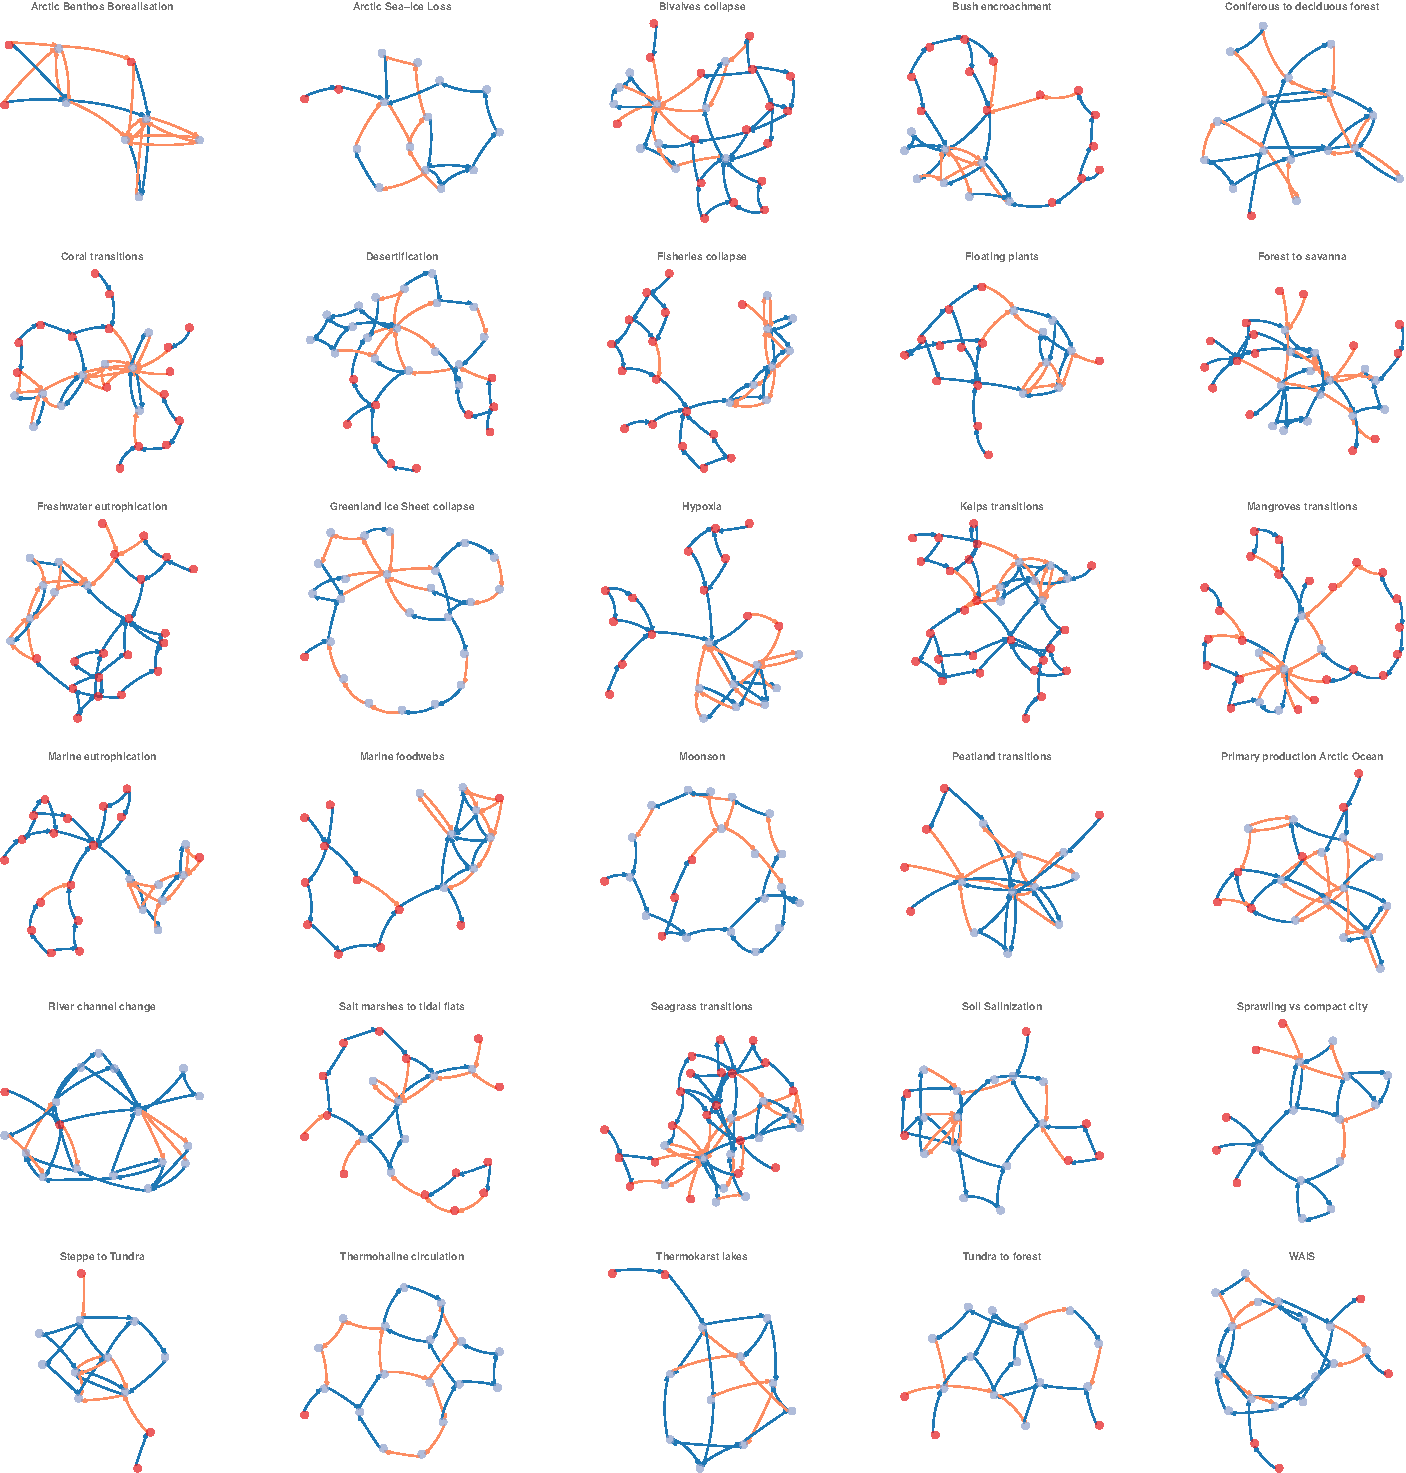
\includegraphics{170830_draftCascadingEffects_files/figure-latex/supp1-1} 

}

\caption{Supplementary figure 1. Causal netoworks for all regime shifts}\label{fig:supp1}
\end{figure}

\pagebreak

\hypertarget{refs}{}
\hypertarget{ref-Sole:2011us}{}
1. Solé, R. V. \emph{Phase Transitions}. (Princeton University Press,
2011).

\hypertarget{ref-Scheffer:2009wl}{}
2. Scheffer, M. \emph{Critical Transitions in Nature and Society}.
(Princeton University Press, 2009).

\hypertarget{ref-Biggs:2015iha}{}
3. Biggs, R. O., Peterson, G. D. \& Rocha, J. C. The Regime Shifts
Database: A framework for analyzing regime shifts in social-ecological
systems. \emph{bioRxiv} (2015).

\hypertarget{ref-Lewontin:1969vh}{}
4. Lewontin, R. C. Meaning of Stability. \emph{Brookhaven Sym Biol}
(1969).

\hypertarget{ref-Carpenter2003rsi}{}
5. Carpenter, S. R. \emph{Regime shifts in lake ecosystems : pattern and
variation}. (2003).

\hypertarget{ref-Scheffer:2012cta}{}
6. Scheffer, M. \emph{et al.} Anticipating Critical Transitions.
\emph{Science} (2012).

\hypertarget{ref-Scheffer:2009p4449}{}
7. Scheffer, M. \emph{et al.} Early-warning signals for critical
transitions. \emph{Nature} (2009).

\hypertarget{ref-Liu:2015go}{}
8. Liu, J. \emph{et al.} Systems integration for global sustainability.
\emph{Science} (2015).

\hypertarget{ref-Scheffer:2003p339}{}
9. Scheffer, M. \& Carpenter, S. Catastrophic regime shifts in
ecosystems: linking theory to observation. \emph{Trends Ecol Evol}
(2003).

\hypertarget{ref-Scheffer:2001uu}{}
10. Scheffer, M., Carpenter, S., Foley, J. A., Folke, C. \& Walker, B.
Catastrophic shifts in ecosystems. \emph{Nature} (2001).

\hypertarget{ref-Boettiger:2013bm}{}
11. Boettiger, C. \& Hastings, A. Tipping points: From patterns to
predictions. \emph{Nature} (2013).

\hypertarget{ref-Hastings:2010p5336}{}
12. Hastings, A. \& Wysham, D. B. Regime shifts in ecological systems
can occur with no warning. \emph{Ecol Lett} (2010).

\hypertarget{ref-Carpenter:2009jr}{}
13. Carpenter, S. R. \emph{et al.} Science for managing ecosystem
services: Beyond the Millennium Ecosystem Assessment. \emph{P Natl Acad
Sci Usa} (2009).

\hypertarget{ref-MAY:1977p3426}{}
14. May, R. Thresholds and breakpoints in ecosystems with a multiplicity
of stable states. \emph{Nature} (1977).

\hypertarget{ref-Holling:1973p6861}{}
15. Holling, C. S. Resilience and stability of ecological systems.
\emph{Annual review of ecology and systematics} (1973).

\hypertarget{ref-Hughes:2013cv}{}
16. Hughes, T. P., Carpenter, S., Rockström, J., Scheffer, M. \& Walker,
B. Multiscale regime shifts and planetary boundaries. \emph{Trends Ecol
Evol} (2013).

\hypertarget{ref-Diaz:2008p199}{}
17. Diaz, R. J. \& Rosenberg, R. Spreading Dead Zones and Consequences
for Marine Ecosystems. \emph{Science} (2008).

\hypertarget{ref-Altieri:2017bl}{}
18. Altieri, A. H. \emph{et al.} Tropical dead zones and mass
mortalities on coral reefs. \emph{P Natl Acad Sci Usa} (2017).

\hypertarget{ref-Zemp:2017dr}{}
19. Zemp, D. C. \emph{et al.} Self-amplified Amazon forest loss due to
vegetation-atmosphere feedbacks. \emph{Nature Communications} (2017).

\hypertarget{ref-Boers:2017ej}{}
20. Boers, N., Marwan, N., Barbosa, H. M. J. \& Kurths, J. A
deforestation-induced tipping point for the South American monsoon
system. \emph{Sci. Rep.} (2017).

\hypertarget{ref-Donges:2015fv}{}
21. Donges, J. F. \emph{et al.} Non-linear regime shifts in Holocene
Asian monsoon variability: potential impacts on cultural change and
migratory patterns. \emph{Climate of the Past} (2015).

\hypertarget{ref-Malik:2011bv}{}
22. Malik, N., Bookhagen, B., Marwan, N. \& Kurths, J. Analysis of
spatial and temporal extreme monsoonal rainfall over South Asia using
complex networks. \emph{Clim Dynam} (2011).

\hypertarget{ref-Clark:2015bj}{}
23. Clark, D. B., Hurtado, J. \& Saatchi, S. S. Tropical Rain Forest
Structure, Tree Growth and Dynamics along a 2700-m Elevational Transect
in Costa Rica. \emph{PLoS ONE} (2015).

\hypertarget{ref-MoruetaHolme:2015fy}{}
24. Morueta-Holme, N. \emph{et al.} Strong upslope shifts in
Chimborazo's vegetation over two centuries since Humboldt. \emph{P Natl
Acad Sci Usa} (2015).

\hypertarget{ref-Bakun:2010p5340}{}
25. Bakun, A., FIELD, D. B., Redondo-Rodriguez, A. \& WEEKS, S. J.
Greenhouse gas, upwelling-favorable winds, and the future of coastal
ocean upwelling ecosystems. \emph{Glob Change Biol} (2010).

\hypertarget{ref-DebraPCPeters:2004ex}{}
26. Peters, D. \emph{et al.} Cross-scale interactions, nonlinearities,
and forecasting catastrophic events. \emph{P Natl Acad Sci Usa} (2004).

\hypertarget{ref-Young:2016kj}{}
27. Young, A. M., Higuera, P. E., Duffy, P. A. \& Hu, F. S. Climatic
thresholds shape northern high-latitude fire regimes and imply
vulnerability to future climate change. \emph{Ecography} (2016).

\hypertarget{ref-Kelly:2015iq}{}
28. Kelly, R., Genet, H., McGuire, A. D. \& Hu, F. S.
Palaeodata-informed modelling of large carbon losses from recent burning
of boreal forests. \emph{Nature Climate Change} (2015).

\hypertarget{ref-Zona:2016hq}{}
29. Zona, D. Biogeochemistry: Long-term effects of permafrost thaw.
\emph{Nature} (2016).

\hypertarget{ref-Alongi:2014kq}{}
30. Alongi, D. M. Carbon Cycling and Storage in Mangrove Forests.
\emph{Ann Rev Mar Sci} (2014).

\hypertarget{ref-Rocha:2015du}{}
31. Rocha, J. C., Peterson, G. D. \& Biggs, R. Regime Shifts in the
Anthropocene: Drivers, Risks, and Resilience. \emph{PLoS ONE} (2015).

\hypertarget{ref-Rocha:2010vv}{}
32. Rocha, J. C. The domino effect: a network analysis of regime shifts
drivers and causal pathways. (Stockholm Resilience Centre, Stockholm
University, 2010).

\hypertarget{ref-Anonymous:2007tc}{}
33. Peters, D. P. C., Sala, O. E., Allen, C. D., Covich, A. \& Brunson,
M. Cascading events in linked ecological and socioeconomic systems.
\emph{FRONTIERS IN ECOLOGY} (2007).

\hypertarget{ref-Krivitsky:2012uo}{}
34. Krivitsky, P. N. Exponential-family random graph models for valued
networks. \emph{Electronic Journal of Statistics} (2012).

\hypertarget{ref-Handcock:2008p5095}{}
35. Handcock, M., Hunter, D., Butts, C., Goodreau, S. \& Morris, M.
statnet: Software tools for the representation, visualization, analysis
and simulation of network data. \emph{J Stat Softw} (2008).

\hypertarget{ref-Hunter:2008vh}{}
36. Hunter, D. R., Handcock, M. S., Butts, C. T., Goodreau, S. M. \&
Morris, M. ergm: A Package to Fit, Simulate and Diagnose
Exponential-Family Models for Networks. \emph{J Stat Softw} (2008).

\hypertarget{ref-Morris:2008ty}{}
37. Morris, M., Handcock, M. S. \& Hunter, D. R. Specification of
Exponential-Family Random Graph Models: Terms and Computational Aspects.
\emph{J Stat Softw} (2008).

\hypertarget{ref-Hunter:2007bq}{}
38. Hunter, D. R. Curved exponential family models for social networks.
\emph{Social networks} (2007).

\hypertarget{ref-RCoreTeam:2012wf}{}
39. R Core Team. R: A Language and Environment for Statistical
Computing. (2017).

\hypertarget{ref-Martin:2015kl}{}
40. Martín, P. V., Bonachela, J. A., Levin, S. A. \& Muñoz, M. A.
Eluding catastrophic shifts. \emph{P Natl Acad Sci Usa} (2015).

\hypertarget{ref-Medeiros:2016vf}{}
41. Medeiros, E. S., Caldas, I. L., Baptista, M. S. \& Feudel, U.
Trapping Phenomenon Attenuates Tipping Points for Limit Cycles. (2016).

\hypertarget{ref-Rocha:2015eea}{}
42. Rocha, J., Yletyinen, J., Biggs, R., Blenckner, T. \& Peterson, G.
Marine regime shifts: drivers and impacts on ecosystems services.
\emph{Phil. Trans. R. Soc. B} (2015).

\hypertarget{ref-Peterson:2016ul}{}
43. Peterson, G. \& Rocha, J. in \emph{Arctic resilience report} (2016).

\hypertarget{ref-Gross:2009jr}{}
44. Gross, T., Rudolf, L., Levin, S. A. \& Dieckmann, U. Generalized
Models Reveal Stabilizing Factors in Food Webs. \emph{Science} (2009).

\hypertarget{ref-Gross:2004uu}{}
45. Gross, T. \& Feudel, U. Analytical search for bifurcation surfaces
in parameter space. \emph{Physica D} (2004).

\hypertarget{ref-Lade:2013iwa}{}
46. Lade, S. J., Tavoni, A., Levin, S. A. \& Schlüter, M. Regime shifts
in a social-ecological system. \emph{Theor Ecol} (2013).

\hypertarget{ref-Keys:2012bo}{}
47. Keys, P. W. \emph{et al.} Analyzing precipitationsheds to understand
the vulnerability of rainfall dependent regions. \emph{BIOGEOSCIENCES}
(2012).

\hypertarget{ref-Singer:2014gj}{}
48. Singer, M. S. \emph{et al.} Herbivore diet breadth mediates the
cascading effects of carnivores in food webs. \emph{P Natl Acad Sci Usa}
(2014).

\hypertarget{ref-Pauly:1998iw}{}
49. Pauly, D., Christensen, V., Dalsgaard, J., Froese, R. \& Torres, F.
Fishing Down Marine Food Webs. \emph{Science} (1998).

\hypertarget{ref-Sterman:2000we}{}
50. Sterman, J. \emph{Business Dynamics: Systems Thinking and Modeling
for a Complex World}. (McGraw-Hill/Irwin, 2000).

\hypertarget{ref-Lane:2008p6781}{}
51. Lane, D. The emergence and use of diagramming in system dynamics: a
critical account. \emph{Systems Research and Behavioral Science} (2008).


\end{document}
